\documentclass{cernatsnote}
\usepackage{physics}
\usepackage{tcolorbox}
\tcbuselibrary{skins}
\usepackage{lipsum}
\usepackage{mathtools}
\usepackage{amsfonts}
\usepackage[colorinlistoftodos]{todonotes}
\usepackage{placeins}
\usepackage{amsmath}
\usepackage{physics}
\usepackage{tcolorbox}
\tcbuselibrary{skins}
\usepackage{lipsum}
\usepackage{amsmath}
\usepackage[T1]{fontenc}
\usepackage{graphicx, subfigure}
\usepackage{fancyhdr}
\usepackage{lmodern}
\usepackage{color}
\usepackage{transparent}
\usepackage{amsfonts}
\usepackage{mathtools}
\usepackage{tikz}
\usetikzlibrary{positioning}
\usepackage{pgfplots}
\pgfplotsset{compat=1.10}
\usepackage{textcomp}
\usepackage{float}
\usepackage{adjustbox} % Used to constrain images to a maximum size 
\usepackage{color} % Allow colors to be defined
\usepackage{enumerate} % Needed for markdown enumerations to work
\usepackage{geometry} % Used to adjust the document margins
\usepackage{amsmath} % Equations
\usepackage{amssymb}
\usepackage{fancyvrb} % verbatim replacement that allows latex
\usepackage{grffile} % extends the file name processing of package graphics 
                         % to support a larger range 
    % The hyperref package gives us a pdf with properly built
    % internal navigation ('pdf bookmarks' for the table of contents,
    % internal cross-reference links, web links for URLs, etc.)
\usepackage{hyperref}
\usepackage{longtable} % longtable support required by pandoc >1.10
\usepackage{tabularx}
\usepackage{epigraph}
\usepackage{quotchap}
\usepackage{lscape}
\usepackage{enumerate}
\usepackage{xpatch}
\usepackage{titletoc}
\usepackage{float}	
\usepackage{xparse}
\NewDocumentCommand{\DIV}{om}{%
  \IfValueT{#1}{\setcounter{#2}{\numexpr#1-1\relax}}%
  \csname #2\endcsname
}

\newtcolorbox{mybox}[3][]
{
  colframe = #2!25,
  colback  = #2!10,
  coltitle = #2!20!black,  
  title    = {#3},
  #1,
}

%\renewcommand{\thesubsection}{\thesection.\alph{subsection}}


\title{Computational Physics – Exercise 4}
\author{Pugazharasu Anancia Devaneyan, Rishi Kumar Senthil Kumar}
\email{\href{pugs@uni-bonn.de}{pugs@uni-bonn.de}, \href{s6risent@uni-bonn.de}{s6risent@uni-bonn.de}}
\date{\today}

\begin{document}
\maketitle

%\begin{abstract}
%This document summarizes ideas from Group theory and representation theory that are vital for the upcoming seminar.
%\end{abstract}
%\\ \\ \\ 

%\begingroup
%\color{black}
%\tableofcontents
%\endgroup

%\section*{Test}
%\section*{Simulation of the 1-D Ising model}

\section{Equations of Motion}
We have the Hamiltonian,
\begin{equation}
\mathcal{H}[\boldsymbol{p}, \boldsymbol{\phi}]=\frac{p_0^2}{2}+\frac{p_1^2}{2}+\frac{p_2^2}{2}+\beta \chi^2(\phi)
\end{equation}
Where,
\begin{equation}
    \chi^2(\phi)=\frac{1}{2} \sum_{i=1}^5 \frac{\left(f_i-f\left(x_i, \phi\right)\right)^2}{\delta f_i^2}
\end{equation}
\begin{equation} \label{3}
    f\left(m_\pi, \boldsymbol{\phi}\right)=\phi_0+\phi_1 m_\pi+\phi_2 m_\pi^2
\end{equation}
\begin{table}[H]
\centering
    \begin{tabular}{c|c|c}
        $m_\pi(\mathrm{GeV})$ & $f_i($ data in $\mathrm{MeV})$ & $\delta f_i($ error in $\mathrm{MeV})$ \\
        \hline 
        $.176$ & 960 & 25 \\
        $.234$ & 1025 & 20 \\
        $.260$ & 1055 & 15 \\
        $.284$ & 1085 & 10 \\
        $.324$ & 1130 & 8 \\
        \hline
    \end{tabular}
\caption{The data we want to fit to.}
\label{tab:data}
\end{table}
Using Hamilton's equations of motion, 
\begin{equation} \label{ham_1}
    \dot{\phi}_{i}=\frac{\partial}{\partial p}_{i} \mathcal{H}
\end{equation}
\begin{equation} \label{ham_2}
    \dot{p}_{i}=-\frac{\partial}{\partial \phi_{i}} \mathcal{H}
\end{equation}
we get
\begin{mybox}{orange}{}
\begin{equation}
    \dot{\phi_{i}} = p_{i} 
\end{equation}
\begin{equation}
    \dot{p}_{0} = - \frac{\beta}{2} . \sum^{5}_{j = 1} \frac{2f(m_{\pi_{j}}, \phi)-f_{j}}{\delta f_{j}}
\end{equation}
\begin{equation}
    \dot{p}_{1} = -\frac{\beta}{2} .  \frac{(1-2m_{\pi_j})f_{j}-2m_{\pi_j}f(m_{pi_{i}, \phi})}{\delta f_{j}}
\end{equation}
\begin{equation}
    \dot{p}_2 = -\frac{\beta}{2} .  \frac{(1-2m^{2}_{\pi_j})f_{j}-2m^{2}_{\pi_j}f(m_{pi_{i}, \phi})}{\delta f_{j}}
\end{equation}
\end{mybox}
\section{Modified Leapfrog Algorithm}
We modify the Leapfrog algorithm to integrate the EOMs. We plot for the convergence in figure \ref{fig:leap}.
\begin{figure}[H]
    \centering
    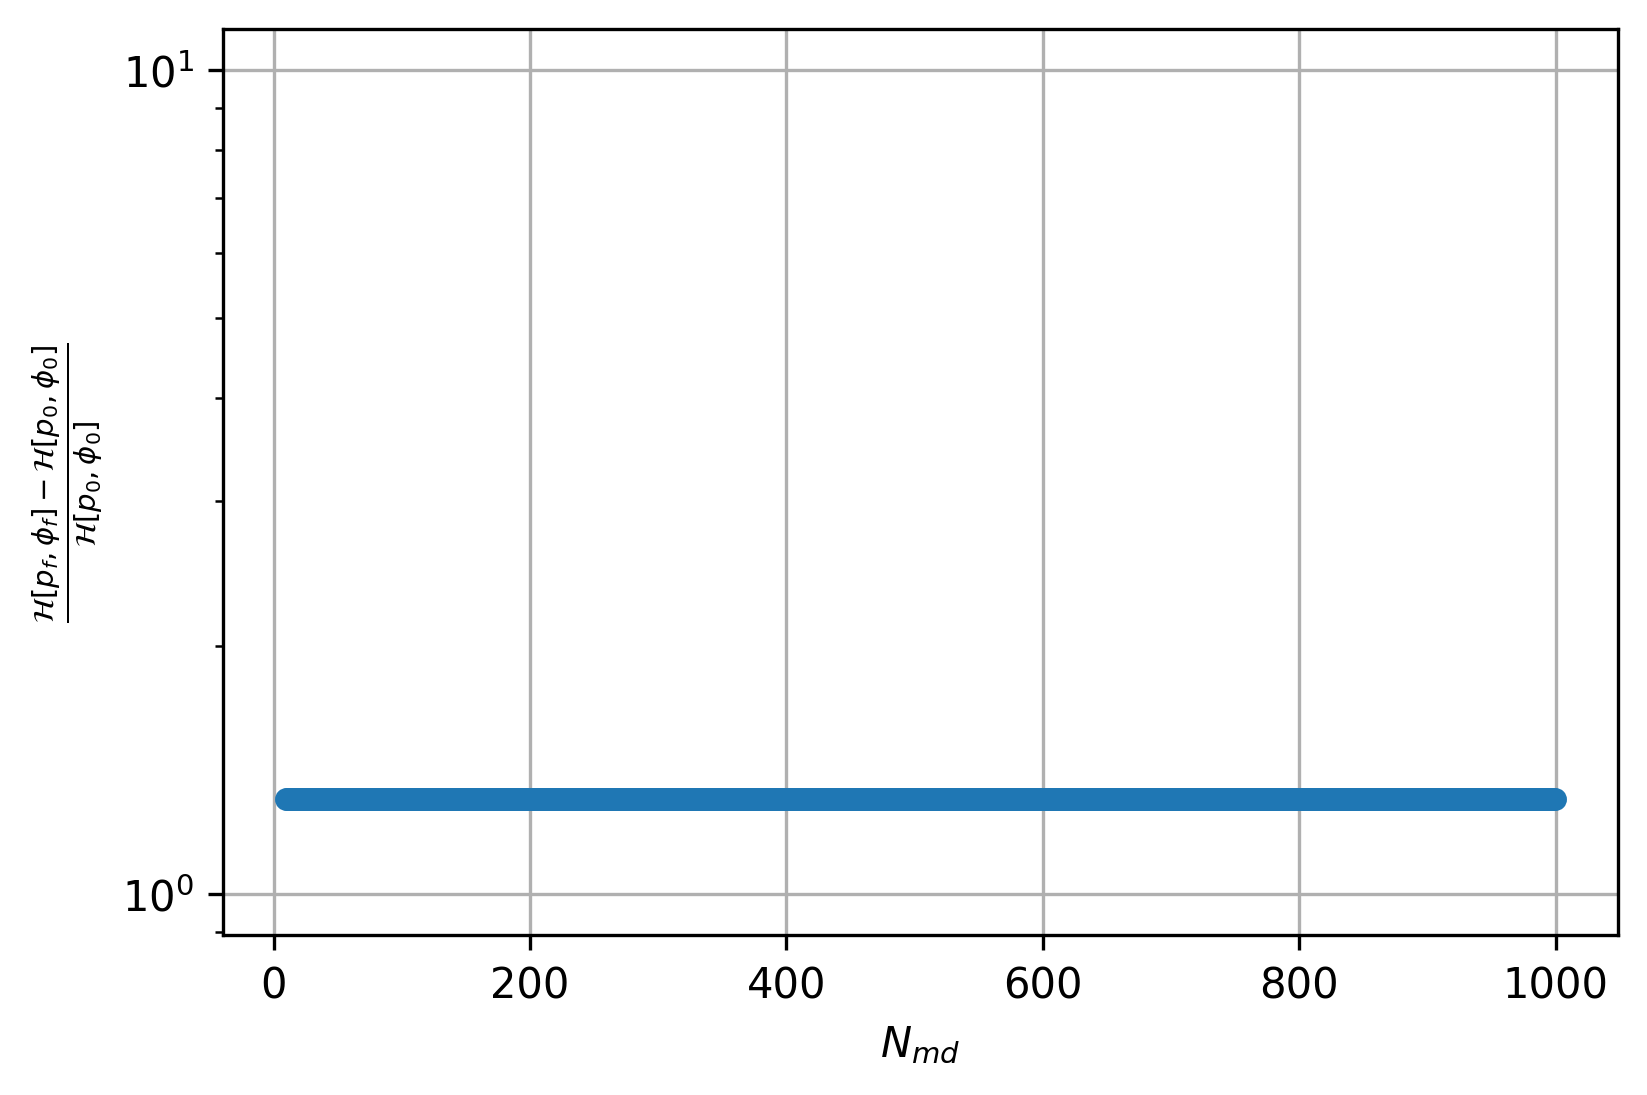
\includegraphics[scale = 0.4]{images/h_v_n.png}
    \caption{Convergence of the leap-frog in in terms of integration steps $N_{md}$.}
    \label{fig:leap}
\end{figure}
\section{Modified Hybrid Monte Carlo}
We coded the HMC for the following case, it can be found at \cite{github}.

\section{Markov Chain as a function of the HMC trajectory}

\section{Finding the best fit}
\section{Mass of the neutron in this chiral limit}
In the chiral limit, the neutron mass corresponds to $\phi_0$ from Eq. (\ref{3}), i.e. the y-intercept.
\bibliographystyle{abbrv}
\bibliography{Bibliography.bib}
\end{document}